\chapter{ALICE}

\section{LHC}
A poca distanza da Ginevra si trova il più grande e il più potente collisore di particelle del mondo \textit{The Large Hadron Collider} (LHC). Ha un raggio complessivo di ben 27 Km ed è stato costruito a partire dal 1998 dall'Organizzazione Europea per la Ricerca Nucleare (CERN). Lo scopo di LHC è quello di avanzare nella conoscenza dell'Universo e dei suoi meccanismi più profondi. Gli esperimenti condotti dal CERN hanno permesso di avere evidenze sperimentali delle principali teorie che spiegano come funziona la materia di cui l'Universo è composto,  a partire dalla scoperta dei bosoni W e Z fino alla scoperta del bosone di Higgs. 
\\LHC è a sua volta composto da varie parti, come mostrato in figura Fig~\ref{fig:CERNcomplex}, che permettono al fascio di particelle finali di avere energie e caratteristiche fondamentali per gli esperimenti che vengono condotti. Si compone da un iniziale acceleratore lineare (Linac2), seguono tre sincrotroni, il Proton Synchrotron Booster (PSB), il Proton Synchrotron (PS) e il Super Protron Synchrotron (SPS) dal quale si ottengono particelle accelerate a 450 $GeV$, che vengono infine iniettate nel LHC dove arrivano ad un'energia di 7 $TeV$ e velocità prossime a quella della luce. \cite{tesi_barbano}
  \captionsetup{justification=centerlast} 
    \begin{figure}[htbp]
        \centering
        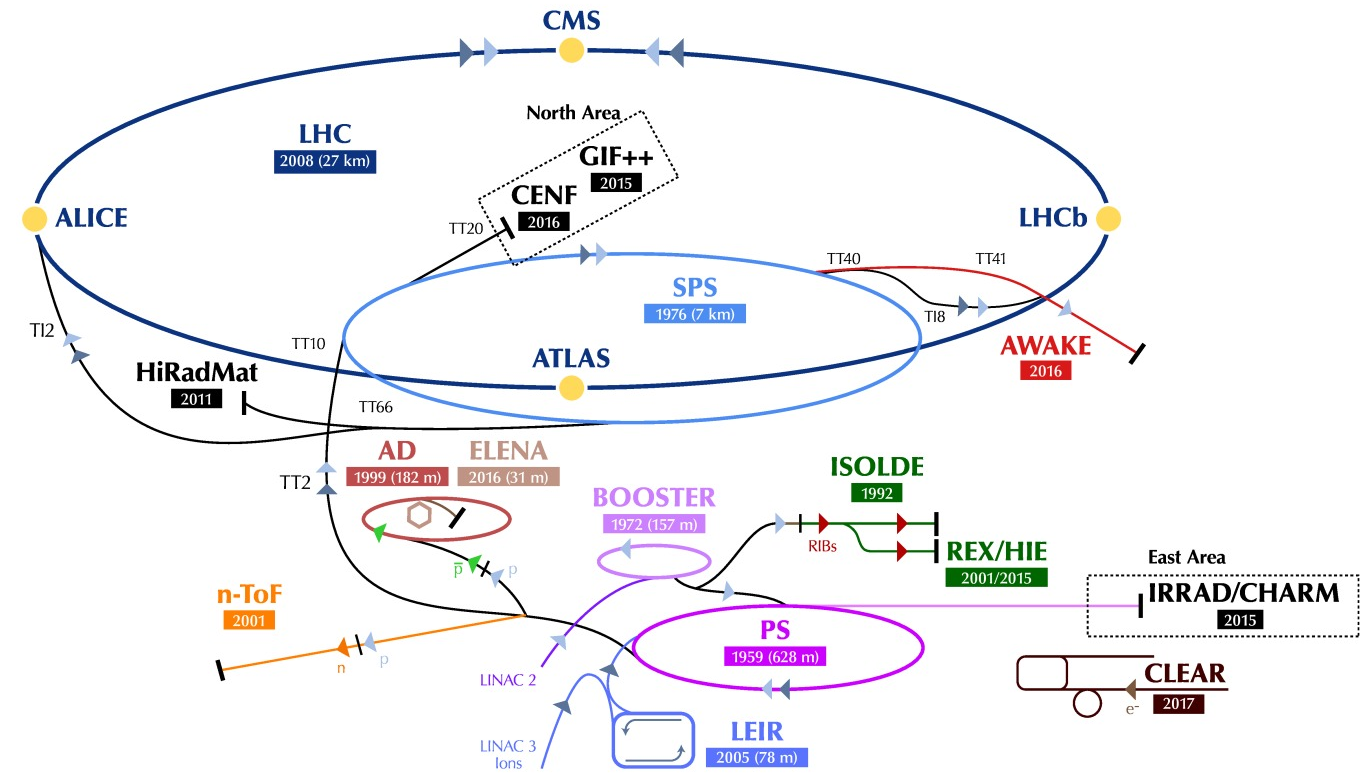
\includegraphics[width=0.8\linewidth]{ALICE/CernComplex_2018.png}        \caption{Complesso dell'intero acceleratore del CERN \\\small{Si vedono  \textcolor{blue}{LHC \textit{Large Hadron Collider}} \textcolor{cyan}{SPS \textit{Super Proton Synchrotron}} \textcolor{purple}{ PS \textit{Proton Synchrotron}} \textcolor{violet}{BOOSTER \textit{ Proton Synchrotron Booster}} LINAC \textit{Linear ACcelerator}} \\{\footnotesize  \textcolor{red}{AD \textit{Antiprotron Decelerator}} \textcolor{green}{ISOLDE \textit{Isotope Separator Online DEvice}}  \textcolor{lightgray}{LEIR \textit{Low Energy Ion Ring}} }}
        \label{fig:CERNcomplex}
    \end{figure}
    
Il fascio di particelle viaggia in un tubo in cui viene fatto l'ultra-vuoto ed è direzionato da dei magneti superconduttivi, che devono essere tenuti alla temperatura di 1.85 $K$.
\\Dal 2008 sono operativi i quattro principali esperimenti di LHC: ALICE, ATLAS, CMS e LHCb. Questi hanno preso dati sia per collisioni protone-protone (\textit{pp}) che per collisioni piombo-piombo (\textit{Pb-Pb}) ed altre. Im questa tesi si utilizzano dati derivanti dall'esperimento ALICE che viene analizzato più nel dettaglio. \cite{sito_cern_LHC} 



\section{ALICE}

L'acronimo ALICE sta per \textit{"A Large Ion Collider Experiment"} e il suo scopo è quello di studiare la materia ad alte densità e alte temperature in uno stato chiamato \textit{quark-gluon plasma} (QGP). ALICE è ottimizzato per lo studio dei prodotti da collisioni ad alte energie di ioni pesanti, casi in cui è possibile studiare il QGP mentre si espande e raffedda. L'obbiettivo è quello di riuscire a comprendere lo stato della materia nei primi microsecondi dopo il Big Bang e in quale modo dal QGP si sono create le particelle di cui è composto ora l'Universo. \cite{sito_cern_ALICE} 
    
    \begin{figure}[htbp]
        \centering
        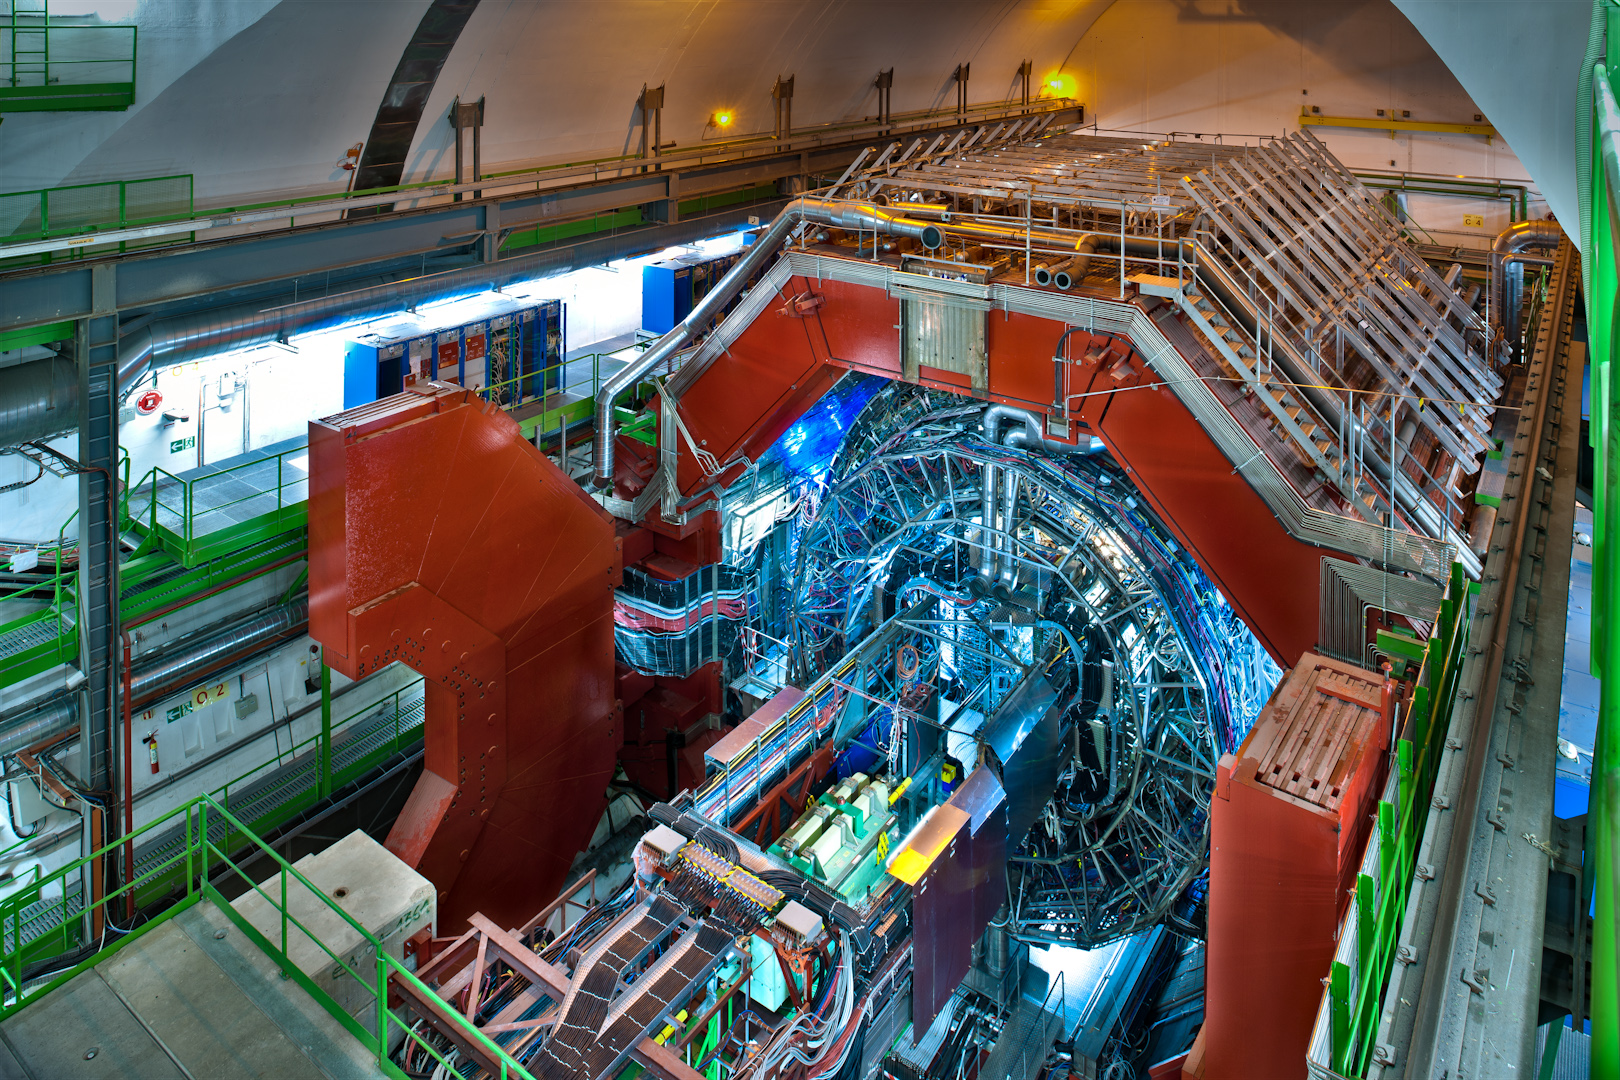
\includegraphics[width=0.6\linewidth]{ALICE/ALICE_LRsaba_CERN_0212_3219.jpg}
        \caption{Foto del rivelatore ALICE}
        \label{fig:ALICEcomplex}
    \end{figure}
    
ALICE è a sua volta composto da molti rivelatori di particelle che permettono di raccogliere dati quali velocità, momento, energia rilasciata ed altri delle particelle create a seguito della collisione dei fasci iniziali. Di seguito si riportano alcuni dettagli sui principali detector di ALICE, i cui dati sono stati utilizzati ai fini di questa tesi.

    \subsection{Inner Tracking System (ITS)} \label{ITS}
    L'\textit{Inner Tracking System} è un rivelatore composto di sei cilindri concentrici di rivelatori in silicone posizionati direttamente attorno al fascio che collide con un raggio minimo di 3.9 $cm$ e massimo di 43.0 $cm$. Viene utilizzato per:
    \begin{itemize}
        \item la determinazione della posizione del vertice primario 
        \item la ricostruzione del vertice secondario di iperoni (come la D$^*$+  )
        \item migliorare la precisione nella determinazione di angolo e momento dati dalla TPC (di cui si parla in seguito al \ref{TPC})
        \item il recupero di particelle che non vengono tracciate dalla TPC a causa delle limitazione sul momento delle particelle che ha la TPC
        \item identificazione di particelle (PID) con basso momento trasverso sfruttando la $dE/dx$
    \end{itemize}
    
    I rivelatori di ITS hanno una risoluzione spaziale di poche decine di micrometri. \cite{tesi_barbano}
    la ricostruzione delle tracce, dei vertici primari e secondari e anche per l'identificazione delle particelle (PID). 

    
    \subsection{Time Projection Chamber  (TPC)} \label{TPC}
    La \textit{Time Projection Chamber}  è il meccansimo migliore per la ricostruzione delle tracce delle particelle tra i rivelatori di ALICE. Anche questo di forma cilindrica si trova Attorno all'ITS, ha un raggio interno di 20 $cm$ e estreno di 250 $cm$, mentre è lungo 500 $cm$ nella direzione del fascio di particelle. Il raggio interno è determinato dalla massima densità di tracce accettabile dal TPC, quello esterno dalla lunghezza minima necessaria per una precisione del 10$\%$ della $dE/dx$. 
     
     \begin{figure}[htbp]
        \centering
        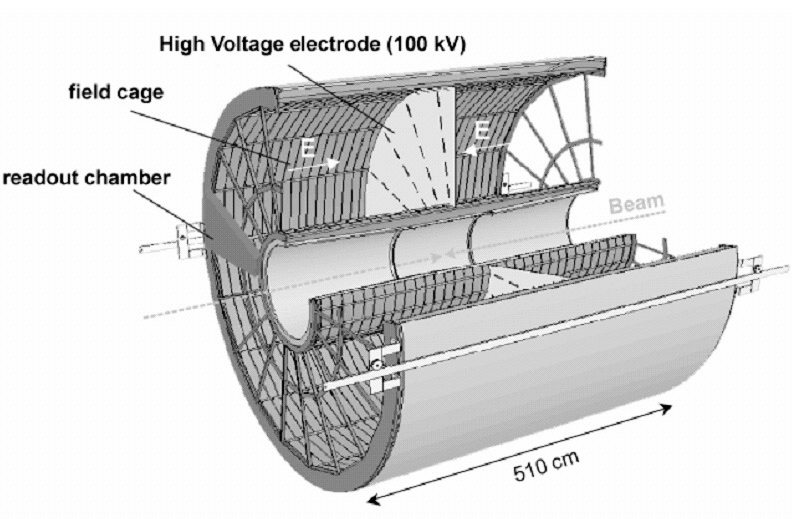
\includegraphics[width=0.6\linewidth]{ALICE/ALICE-TPC-detector.png}
        \caption{Schema della Time Projection Chamber di ALICE}
        \label{fig:TPCcomplex}
    \end{figure}
    
    La camera del TPC è riempita con una miscela di gas, originariamente erano 90$\%$ di $Ne$ e 10$\%$ di $CO_2$, poi è stato aggiunto un 5$\%$ di $N_2$. Questa miscela di gas serve per trasportare gli elettroni di ionizzazione creati dal passaggio della particella da tracciare. Gli elettroni di ionizzazione vengono accelerati dal campo elettrico creato dagli elettrodi della TPC per arrivare alle placche esterne che permettono di registrare il segnale. \cite{Collaboration_2008_ALICE}
    \\La TPC è utilizzata per misurare il momento delle particelle, che viene ricavato dalla curvatura delle tracce ricostruite, causata dal campo magnetico della TPC. Inoltre si utilizza su un vasto range di momenti la PID, questo è possibile grazie alla misura della perdita di energia specifica ( $dE/dx$ ), la carica e il moemnto della particella. Si confrontano i dati con i valori della Bethe-Bloch per identificare la particella considerata. Per calori del momento trasverso $p_T$ minori o uguali ad 1 $GeV/c$  la distinzione tra le particelle è chiara, per valori di $p_T$ più alti si usa la PID in modo statistico. 
    
    \begin{figure}[htbp]
        \centering
        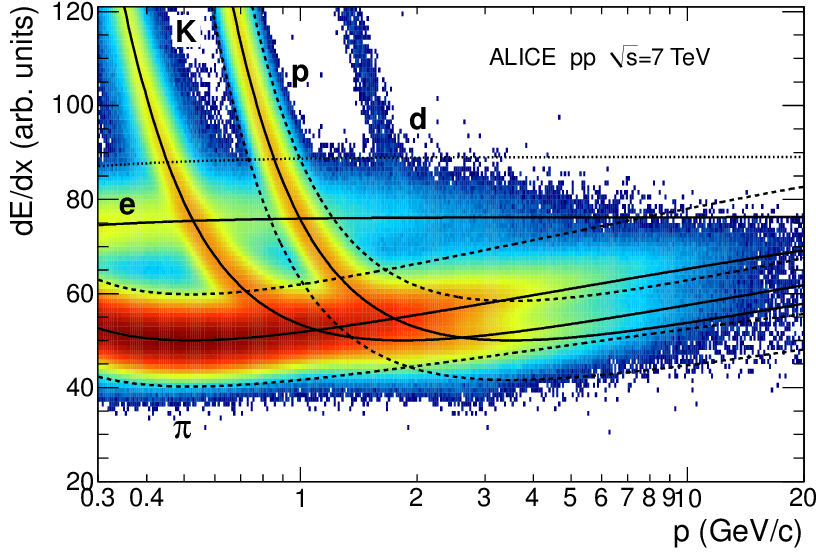
\includegraphics[width=0.6\linewidth]{ALICE/Specific-energy-loss-in-the-TPC.png}
        \caption{ Perdita di energia specifica nela TPC in funzione del momento, sono riportate anche gli andamenti della Bethe-Bloch per vari tipi di particelle.}
        \label{fig:BBnellaTPC}
    \end{figure}
    
    
    
    
    
    